\documentclass[handout]{beamer}

\mode<presentation>
{
  \usetheme{umbc1}
  \setbeamercovered{transparent}
}

\usepackage[english]{babel}
\usepackage[latin1]{inputenc}
\usepackage[T1]{fontenc}
\usepackage{amsmath}

\usepackage[]{datatool, filecontents}
\DTLsetseparator{=}
\DTLloaddb[noheader, keys={key,value}]{values}{./values.dat}
\newcommand{\var}[1]{\DTLfetch{values}{key}{#1}{value}}
\newcommand\Tstrut{\rule{0pt}{2.6ex}}       % "top" strut
\newcommand\Bstrut{\rule[-0.9ex]{0pt}{0pt}} % "bottom" strut
\newcommand{\TBstrut}{\Tstrut\Bstrut} % top&bottom struts

\usepackage{tabularray}

\title[RMP v\var{version}]
{Robot Motion Planning}

\subtitle
{Classic Path Planning Algorithms}

\author[Narayanan]
{A.~Narayanan\inst{1}}

\institute[Technical University of Munich]
{
  \inst{1}
  Department of Informatics\\
}

\subject{Slides}
\date{}

\AtBeginSubsection[]
{
  \begin{frame}<beamer>{Outline}
    \tableofcontents[currentsection,currentsubsection]
  \end{frame}
}

\begin{document}
\begin{frame}
    \titlepage
  \end{frame}
  
  \begin{frame}{Outline}
    \tableofcontents
  \end{frame}

  \section{Overview of Classic Path Planning Approaches}

  \begin{frame}
    \begin{itemize}
        \item \textbf{Roadmap} \pause

        Represent the connectivity of the free space by 1-D Curves \pause

        \item \textbf{Cell Decomposition} \pause

        Decompose the free space into simple cells and represent the connectivity of the free space by adjacency graph of these cells \pause

        \item \textbf{Potential Field} \pause

        Define a potential function over the free space that has a global minimum at the goal and follow the steepest descent of the potential function
    \end{itemize}
  \end{frame}

  \section[Roadmaps]{Roadmaps}

  \begin{frame}{Roadmaps}
    \begin{itemize}
      \item construct a \texttt{map} once and then use that map to plan subsequent paths more quickly \pause
      \item Topological maps aim at representing environments with graphlike structures \pause
      \item \textbf{Roadmaps} are a type of topological map embedded in free space where each node corresponds to a specific location and an edge corresponds to a path between neighboring locations \pause
    \end{itemize}
  
    

    \centering
    find path from $q_{start}$ to roadmap $\rightarrow$ \pause traverse roadmap to vicinity of goal $\rightarrow$  \pause find path from roadmap to the $q_{goal}$
  
  \end{frame}

  \begin{frame}{Definition}
    
    A union of one-dimensional curves is a roadmap RM if for all $q_{start}$ and $q_{goal}$ in $\mathcal{Q}_{free}$ that can be connected by a path, the following properties hold:
    \begin{enumerate}
      \item \textbf{Accessibility}: there exists a path from $q_{start} \in \mathcal{Q}_{free}$ to some $q'_{start}  \in RM$,
      \item \textbf{Departability}: there exists a path from some $q'_{goal} \in RM$ to $q_{goal} \in \mathcal{Q}_{free}$, and
      \item \textbf{Connectivity}: there exists a path in $RM$ between $q'_{start}$  and $q'_{goal}$   .
    \end{enumerate}

  \end{frame}

  \begin{frame}{Advantages}
    
    \begin{enumerate}
      \item Efficient method of path planning in the configuration space. It moves a large part of processing to offline. 
      \item Just need to connect $q_{init}$, $q_{goal}$ to roadmap online.
      \item Finding a path is like searching in a roadmap.
    \end{enumerate}

  \end{frame}

  \subsection[Visibility Maps]{Visibility Maps}

  \begin{frame}{Visibility Graph}

    \begin{columns}
      \begin{column}[]{0.4\textwidth}
        Assume a polygonal configuration space with obstacles approximated as polygons, with the nodes $v_{i}$ of the graph consisting of $q_{start}$, $q_{goal}$ and all obstacle vertices
      \end{column}
      \begin{column}[]{0.6\textwidth}
        \begin{center}
        \begin{figure}
          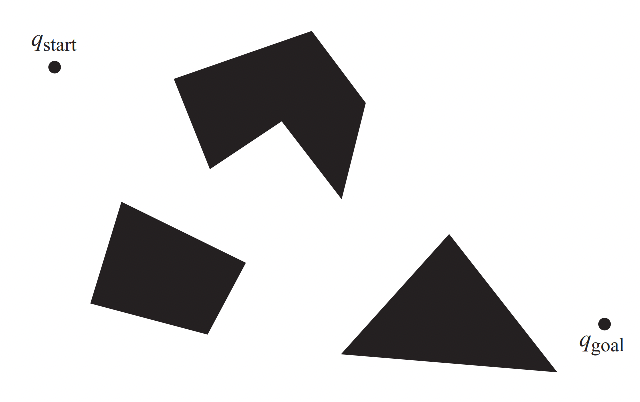
\includegraphics[width=60mm]{fig/fig_02_poly_cofig_space.png}
          \caption{A polygonal config space with start and goal}
          \label{fig:fig02}
        \end{figure}
       \end{center}
      \end{column}
    \end{columns}
    
  \end{frame}

  \begin{frame}{Visibility Graph}

    \begin{columns}
      \begin{column}[]{0.4\textwidth}
        The graph edges $e_{ij}$ are straight-line segments that connect two line-of-sight nodes $v_{i}$ and $v_{j}$

        \centering
        \begin{table}
          \begin{tblr}{|c|}
            \hline
            \textbf{Complexity:} $O(n^{2})$ \TBstrut\\
            \hline
          \end{tblr}
        \end{table}
        
      \end{column}
      \begin{column}[]{0.6\textwidth}
        \begin{center}
        \begin{figure}
          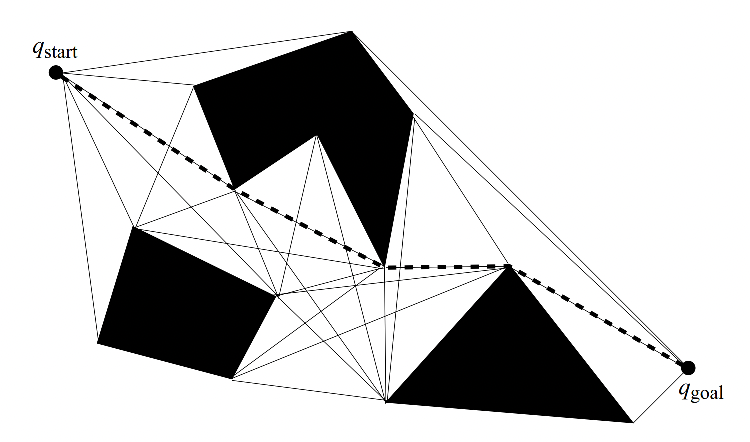
\includegraphics[width=60mm]{fig/fig_03_visibility_graph.png}
          \caption{The Visibility graph}
          \label{fig:fig03}
        \end{figure}
       \end{center}
      \end{column}
    \end{columns}
    
  \end{frame}

  \begin{frame}{Reduced Visibility Graph}

  the visibility graph has many needless edges. The use of supporting and separating lines can reduce the number of edges.

    \begin{columns}
      \begin{column}[]{0.4\textwidth}
        \begin{center}
          \begin{figure}
            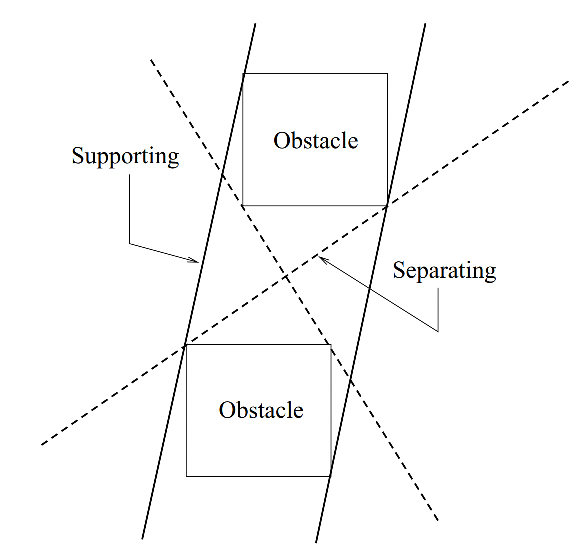
\includegraphics[width=40mm]{fig/fig_04_supporting_separating_segments.png}
            \caption{Supporting and Separating Line Segments}
            \label{fig:fig04}
          \end{figure}
         \end{center}
      \end{column}
      \begin{column}[]{0.6\textwidth}
        \begin{center}
        \begin{figure}
          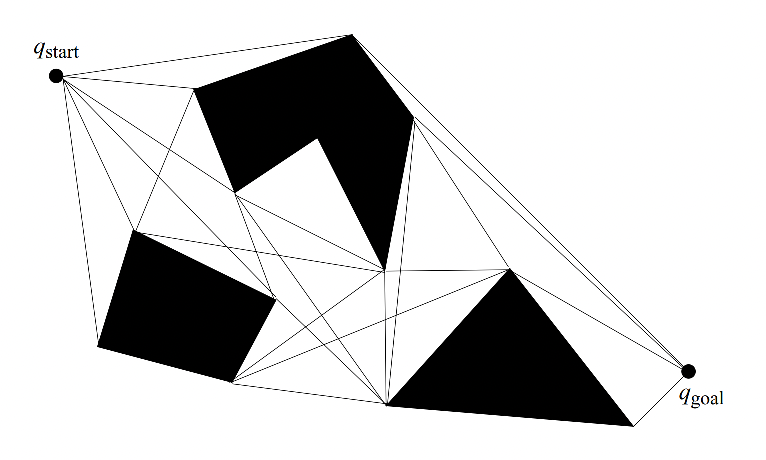
\includegraphics[width=60mm]{fig/fig_05_reduced_visibility_graph.png}
          \caption{Reduced Visibility graph}
          \label{fig:fig05}
        \end{figure}
       \end{center}
      \end{column}
    \end{columns}
    
  \end{frame}

  \begin{frame}
    \frametitle{Rotational Plane Sweep Algorithm}
  
    
  
  \end{frame}

  \subsection[Voronoi Diagrams]{Generalized Voronoi Diagrams}

  \begin{frame}
    \frametitle{Generalized Voronoi Diagrams}
    The \textbf{Generalized Voronoi Diagram} (\textbf{GVD}) is the set of points where the distance to the two closest obstacles is the same.
    \begin{center}
      \begin{figure}
        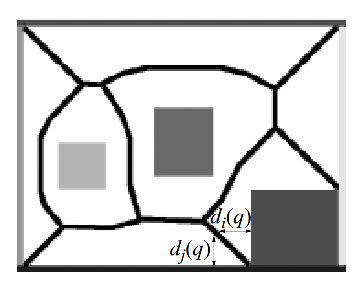
\includegraphics[width=60mm]{fig/fig_06_gvd.png}
        \caption{Voronoi Diagram}
        \label{fig:fig06}
      \end{figure}
     \end{center}
     \centering
     \begin{table}
       \begin{tblr}{|c|}
         \hline
         \textbf{Complexity:} $O(n \log(n))$ \TBstrut\\
         \hline
       \end{tblr}
     \end{table}
  
  \end{frame}

  \begin{frame}
    \frametitle{Construction of the GVD}
    \begin{center}
      \begin{figure}
        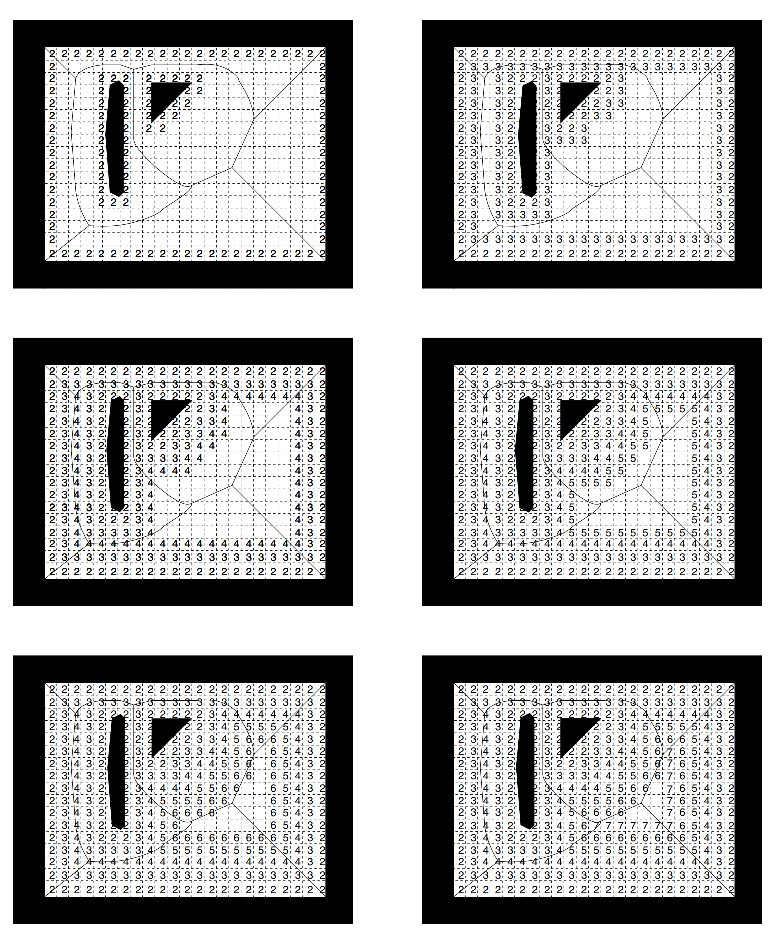
\includegraphics[width=55mm]{fig/fig_07_brushfire.png}
        \caption{The \textbf{Brushfire algorithm} uses a grid to approximate distance}
        \label{fig:fig07}
      \end{figure}
     \end{center}
  
  \end{frame}

  \section[Cell Decompositions]{Cell Decomposition}

  \begin{frame}
    \frametitle{Cell Decompositions}
    The main idea is to decompose the free space into simple cells and represent the connectivity of the free space F by the adjacency of these cells. It is called an exact cell decomposition if the union of all cells is exactly F, meaning there is no overlap between cells.
  \end{frame}

  \subsection{Trapeziodal decomposition}

  \begin{frame}
    \frametitle{Trapeziodal Decomposition}
    \begin{itemize}
      \item The free space is bounded by polygons and C-Space obstacles are poygon shaped
      \item decompose the space into trapezoidal triangle cells
      \item connect every neighboring centered point in every neighboring cells that dont intersect with obstacles (\textbf{Adjacency graph})
    \end{itemize}
    \alert{Problems:} there are a lot of useless small cells that could be aggregated to avoid long and less efficient paths
  
  \end{frame}

  \subsection{Boustrophedon Decomposition}

  \begin{frame}
    \frametitle{Boustrophedon Decomposition}
    \begin{itemize}
      \item Consider the vertices at which a vertical line can be extended both up and down in free space i.e. the critical points
      \item set boundary lines at critical points
      \item Then, an exhaustive walk through the critical
      points is performed in order to obtain a connectivity graph
    \end{itemize}    
  
  \end{frame}

  \section[Potential Field]{Potential Field}

  \begin{frame}
    \frametitle{Potential Field Method}
    \begin{itemize}
      \item The C-space is turned into a potential field, where the obstacles are surrounded by a repulsive field
      \item The goal location by an attractive field. To navigate, the robot applies a force proportional to the negative gradient of the field - this is called gradient descent.
      \item \textbf{Advantage:} potential field methods are easy to compute.
      \item \textbf{Disadvantage:} They can suffer from local minima (where robot gets stuck), and they don't consider dynamic constraints in their initial form (forces can be too high).
    \end{itemize}
  \end{frame}

  \begin{frame}
    \frametitle{The Attractive Potential}
    \begin{itemize}
      \item we could use \texttt{Conic Potential} - When numerically implementing this method, gradient descent may have "chattering" problems since there is a discontinuity in the attractive gradient at the origin. 
      \item or we could use \texttt{Quadratic Potential} - grows without bound as $q$ moves away from $q_{goal}$. If $q_{start}$ is far from $q_{goal}$, this may produce a desired velocity that is too large
      \item Solution - conic potential attracts the robot when it is very distant from $q_{goal}$ and the quadratic potential attracts the robot when it is near $q_{goal}$. 
    \end{itemize}

    \centering

    \begin{equation}
      U_{att}(q) =
        \begin{cases}
          \frac{1}{2}\zeta d^{2}(q, q_{goal})  & d(q, q_{goal} \leq d^{*}_{goal}\\
          d^{*}_{goal}\zeta d(q, q_{goal}) - \frac{1}{2}\zeta (d^{*}_{goal})^{2} & d(q, q_{goal} > d^{*}_{goal}\\
        \end{cases}       
    \end{equation}

  \end{frame}

\end{document}